\documentclass[conference]{IEEEtran}
% 功能概述：本文档是 SpectraExpert 最终稿的唯一 LaTeX 入口，使用 IEEE Conference Template 组织正文、公式、图表和参考文献。
% 主要职责：汇编十页最终稿；围绕理论到实验域偏移、当前模型原理及同协议证据组织正文。
% 代码库关系：引用 figures/、ref/ref.bib 和未经修改的 IEEEtran.cls；由 latexmk 编译到 build/，稳定产物复制到 ../output/pdf/。
% 内容版本：2026-09-09 用户授权更新实验内容；新指标以已归档 JJ 结果为准，旧 PDF 仅为历史来源。
\usepackage{cite}
\usepackage[T1]{fontenc}

\usepackage{multirow}
\usepackage{booktabs}
\usepackage{balance}
\usepackage{hyperref}
\usepackage{amsmath,amssymb,amsfonts}
\usepackage{algorithmic}
\usepackage{graphicx}
\usepackage{textcomp}
\usepackage{xcolor}
\usepackage{colortbl}
% 功能概述：统一 camera-ready 结果表的视觉样式，复用早期 IEEE 主表的深蓝表头及四色方法分组。
% 主要职责：PaperTableSetup 设置局部字号和间距；PaperHead 设置白色粗体表头；PaperGroup 和 PaperNote 分别排版分组及说明。
% 代码库关系：由 main.tex 在导言区载入，供 latest_results、native_results、historical_results 的编号表调用。
% 输入输出与副作用：只影响显式调用的表格；颜色无数值排名含义，不改动指标、样本或统计口径。
\usepackage{tabularx}
\usepackage{caption}
\captionsetup[table]{font=small,labelfont=bf,skip=6pt,justification=centering}
\definecolor{HdrBg}{HTML}{1E3A5F}
\definecolor{RetBg}{HTML}{DBEAFE}
\definecolor{DirBg}{HTML}{DCFCE7}
\definecolor{KnwBg}{HTML}{FEF3C7}
\definecolor{AgtBg}{HTML}{FCE7F3}
\definecolor{SecTxt}{HTML}{1E293B}
\newcommand{\PaperTableSetup}[1]{%
  #1\renewcommand{\arraystretch}{1.38}%
  \setlength{\tabcolsep}{5pt}%
  \setlength{\aboverulesep}{0pt}%
  \setlength{\belowrulesep}{0pt}%
  \arrayrulecolor{HdrBg}}
\newcommand{\PaperHead}[1]{{\color{white}\bfseries #1}}
\newcommand{\PaperGroup}[3]{%
  \rowcolor{#2}\multicolumn{#1}{l}{\color{SecTxt}\bfseries\itshape #3}\\}
\newcommand{\PaperNote}[1]{%
  \par\vspace{4pt}\begin{minipage}{\linewidth}%
  \footnotesize\raggedright #1\end{minipage}}

\def\BibTeX{{\rm B\kern-.05em{\sc i\kern-.025em b}\kern-.08em
    T\kern-.1667em\lower.7ex\hbox{E}\kern-.125emX}}

\hypersetup{
  hidelinks,
  pdftitle={SpectraExpert: Expert-Like Reasoning Agent for Spectrum-Based Molecular Identification},
  pdfauthor={Denghong Luan, Zaifan Lu, Wenjie Wang, Wei Hu, and Jun Jiang},
  pdfsubject={Raman spectrum-based molecular identification},
  pdfkeywords={Retrieval-augmented reasoning, contrastive learning, raman spectroscopy, molecular identification, large language models}
}

% 作者已确认插入训练方法图。
\newcommand{\SpectraExpertFinalTrainingArtwork}{}
\begin{document}


\title{SpectraExpert: Expert-Like Reasoning Agent for Spectrum-Based Molecular Identification}
\author{
\IEEEauthorblockN{
Denghong Luan\IEEEauthorrefmark{1},
Zaifan Lu\IEEEauthorrefmark{2},
Wenjie Wang\IEEEauthorrefmark{1},
Wei Hu\IEEEauthorrefmark{3},
Jun Jiang\IEEEauthorrefmark{3}
}

\IEEEauthorblockA{
\IEEEauthorrefmark{1}
School of Artificial Intelligence and Data Science,
University of Science and Technology of China\\
Hefei, China\\
dhluan@mail.ustc.edu.cn, wenjiewang96@gmail.com
}

\IEEEauthorblockA{
\IEEEauthorrefmark{2}
School of Physical Science,
University of Science and Technology of China\\
Hefei, China\\
elenwath\_lzf@mail.ustc.edu.cn
}

\IEEEauthorblockA{
\IEEEauthorrefmark{3}
School of Chemistry and Materials Science,
University of Science and Technology of China\\
Hefei, China\\
\{weihulp, jiangj1\}@ustc.edu.cn
}
}


\maketitle


\begin{abstract}
Raman molecular identification requires both retrieval across theory--experiment spectral mismatch and discrimination among similar structures. SpectraExpert combines domain-adapted retrieval with constrained large language model (LLM) selection and optional spectroscopic evidence. A coverage-aware spectral Transformer learns from experimental--theoretical pairs, source-dependent curve proxies and identity-aware hard negatives. On 200 experimental queries against 10,000 reference structures, five-seed Exact@10 reaches 53.60\% $\pm$ 2.36\%, compared with 46.30\% $\pm$ 5.22\% for paired training. Development gains are consistent, but the paired test-gain interval includes zero. With frozen single-seed candidates and legacy knowledge, five LLMs achieve 16.5--29.0\% exact identification after documented output recovery. Claude selects 58 of 103 retrievable targets correctly, compared with 41 exact matches from retrieval top-1. Thus, both missed retrievals and incorrect selections limit final accuracy. DeepSeek ablations show no stable additional knowledge benefit. These findings separate retrieval and selection failures in closed-library transfer to unseen experimental spectra of known molecular identities.
\end{abstract}
\begin{IEEEkeywords}
Raman spectroscopy, domain adaptation, contrastive retrieval, molecular identification, retrieval-augmented reasoning
\end{IEEEkeywords}

% 提前提交跨栏流程图，使其排在第二页页首；方法段落仍保留对应说明。
\begin{figure*}[!t]
\centering
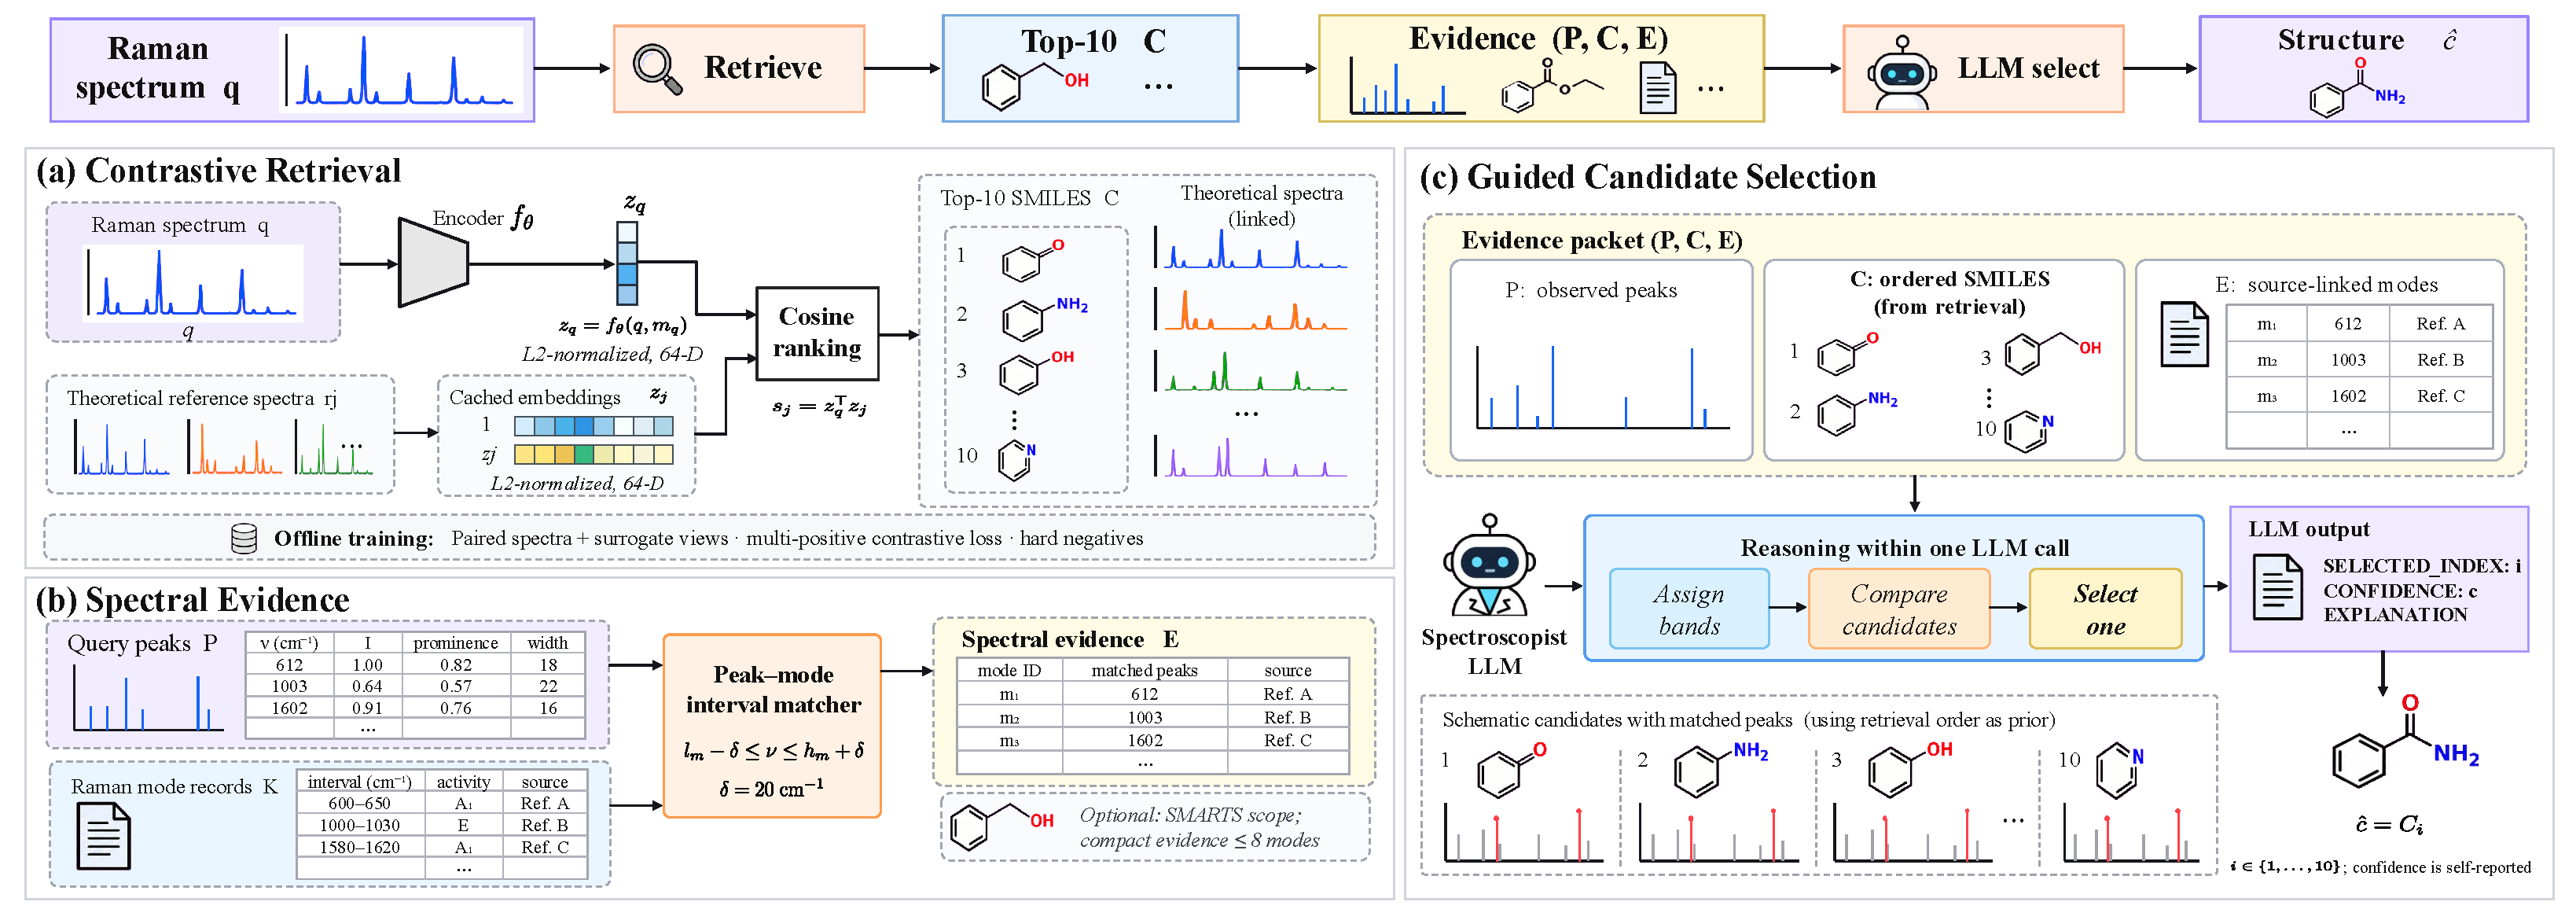
\includegraphics[width=\textwidth]{figures/spectraexpert_agent_workflow.pdf}
\caption{SpectraExpert workflow for Raman-based molecular identification. (a) A shared coverage-aware encoder maps the query and cached theoretical references to normalized 64-dimensional embeddings for top-ten retrieval. Offline training combines paired spectra, surrogate views, a multi-positive contrastive loss and hard negatives. (b) Observed peaks $P$ are matched to mode intervals to construct spectral evidence $E$. The illustrated 15-mode development branch uses a 20\,cm$^{-1}$ tolerance; Test-200 uses the legacy library described in Section~\ref{sec:selection}. (c) The LLM compares ordered candidate SMILES $C$ using $P$ and optional $E$, then selects one candidate index. Confidence is self-reported and does not trigger structural edits. Candidate spectra, molecular sketches, numerical entries and Ref.\ A--C labels are schematic; candidate spectra are not provided to the LLM.}
\label{fig:domain_pipeline}
\end{figure*}

\section{Introduction}\label{sec:intro}
Raman spectra connect molecular vibrations with chemical structure~\cite{raman1928change,kudelski2008analytical}, supporting chemical and biological analysis~\cite{shipp2017raman}. Identifying a molecule from a measured spectrum, however, requires more than matching peak positions. Theoretical references and experimental measurements differ in frequency calibration, band width, relative intensity and spectral coverage. Chemically related structures may also share prominent bands. A retrieval system must first place the correct identity in a manageable candidate set; a subsequent decision must distinguish that identity from plausible alternatives.

These difficulties are easy to conflate. A language model cannot recover a missing target through candidate selection, while a high top-ten retrieval rate does not demonstrate reliable final identification. Direct SMILES generation adds a separate burden: valid chemical syntax does not guarantee agreement with the observed spectrum. We therefore formulate SpectraExpert as a controlled retrieve--analyze--select system, and evaluate retrieval coverage separately from the quality of the final choice.

Our primary technical focus is theory--experiment domain shift. Training only with perturbed theoretical spectra need not reproduce experimental distortions. We combine real experimental--theoretical pairs with a low-dimensional curve proxy fitted separately for each theoretical source. Randomized views around this proxy model variation within a source; missing-data masks prevent unmeasured spectral regions from acting as observed zero intensity. An identity-aware contrastive objective aligns the two domains without treating repeated references of the same structure as negatives. Hard negatives then concentrate training on incorrect structures that remain spectrally confusable.

After retrieval, the system presents ten canonical structures and the experimental peak table to an LLM. Spectroscopic rules can supply additional, explicitly limited evidence. The deployed decision is constrained to a supplied candidate: the earlier unrestricted structural modification policy is disabled because its confidence trigger did not reliably improve molecular similarity. This design preserves a measurable retrieval ceiling and permits paired comparisons with retrieval alone, simple rule coverage and a learned linear reranker.

Our contribution is a domain-adaptation procedure and an evaluation protocol that distinguish retrieval coverage from final identification. Controlled curve-proxy and hard-negative experiments assess retrieval across five paired training seeds. Common-query comparisons then assess LLM selection and knowledge effects using frozen candidates. The benchmark represents every test identity in the theoretical library while withholding its experimental spectra from training. This design tests transfer to new measurements of known identities and makes each stage's contribution separately measurable.

\section{Related Work}\label{sec:related}
\subsection{Spectral Representations and Molecular Retrieval}
Learned spectrum prediction~\cite{zou2023deep} and the computed Raman/IR extension of ChEMBL~\cite{liang2025dataset} expand access to theoretical spectra. These resources do not by themselves establish transfer to experimental measurements. RamanBench documents cross-dataset generalization difficulties across Raman classification and regression tasks~\cite{koddenbrock2026ramanbench}; our focus is exact molecular retrieval.

Learned spectral representations, including RamanNet~\cite{ibtehaz2023ramannet}, complement direct curve similarity by extracting task-dependent features. Contrastive learning~\cite{chen2020simple} provides a natural way to make corresponding observations close while separating alternatives. The central issue here is which observations are treated as corresponding: two synthetic views alone do not impose alignment with an experimentally measured spectrum.

VibraCLIP embeds molecular graphs and vibrational spectra in a shared space~\cite{vibraclip}; Vib2Mol combines spectrum-to-structure retrieval and generation~\cite{vib2mol}. These methods are direct comparators for molecular identification, and we evaluate their available checkpoints on the same experimental queries. Our encoder uses shared spectral weights on both sides, with paired adaptation, explicit coverage treatment and train-only negative mining. We do not claim that this standard backbone or contrastive loss family is novel. The comparison also does not equalize adaptation resources: SpectraExpert receives the experimental training pairs defined below, whereas the collected competitor runs use their available pretrained checkpoints.

\subsection{Knowledge-Guided Scientific Reasoning}
Chain-of-thought prompting studies intermediate reasoning steps~\cite{wei2022chain}, while ChemLLM incorporates structured chemical knowledge into dialogue~\cite{zhang2024chemllm}. ChemCrow integrates chemistry tools~\cite{m2024augmenting}, and Coscientist combines language models with tools for autonomous chemical experimentation~\cite{boiko2023autonomous}. These systems motivate modular scientific assistants, but do not establish that verbal explanations improve Raman candidate selection.

Modular systems such as MRKL, Toolformer and ReAct combine language models with external knowledge or tools~\cite{karpas2022mrkl,schick2023toolformer,yao2023react}. MatExpert applies a retrieval--transition--generation workflow to materials design~\cite{ICLR2025_7d6850f4}. SpectraExpert adopts this general decomposition for Raman identification; assembling these components is not itself a new reasoning algorithm. Our measurable question is whether spectral evidence improves selection after the candidate set has been frozen.

Group-frequency references associate vibrational regions with possible functional groups~\cite{socrates2004infrared,nakamoto2008infrared}. Their assignments depend on molecular context, so a matched interval is supporting evidence rather than proof of a complete structure. The current mode-level controls use 15 Raman records traceable to a technical reference~\cite{horibaRATN18}. We distinguish these records from the broader legacy knowledge library and evaluate rules with and without an LLM. MolSpectLLM~\cite{shen2025specmol} is relevant to spectroscopy-grounded molecular learning, but the collected artifacts contain no compatible Raman evaluation; its reported results are not substituted for measurements on our benchmark.

% 功能概述：解释最终稿中实际评测的理论到实验 Raman 域适配模型。
% 主要职责：给出覆盖掩码、来源代理、矩形多正样本损失、困难负样本及候选选择的数学定义。
% 代码库关系：由 main.tex 引入；实现对应 scripts/raman_domain_experiment.py 和 raman_top10_experiment.py。
% 图稿状态：保留 main.tex 中全流程图；作者已确认插入精简版训练机制图。
\section{Problem and Domain-Adaptation Method}\label{sec:method}
\subsection{Closed-Library Identification and Its Two Bottlenecks}
Let $\mathcal{D}=\{(y_j,m_j,c_j,s_j)\}_{j=1}^{M}$ be a library of theoretical spectra $y_j$, coverage masks $m_j$, full molecular identities $c_j$ and theoretical sources $s_j$. An experimental query $(x,m_x)$ has a target identity $c^\star$ in the library. Canonical/isomeric SMILES define exact identity, retaining stereochemistry and isotopes. A separate molecular-group key removes stereochemistry and isotopes after selecting the largest fragment; it is used for split protection and equal weighting of repeated measurements, not for exact-match scoring.

The encoder $f_\theta$ maps a spectrum and its mask to a unit vector. Similarity is $f_\theta(x,m_x)^\top f_\theta(y_j,m_j)$. We rank one fixed reference per unique structure and retain $K=10$ candidates, denoted $\mathcal{C}_{10}(x)$. Keeping a single indexed reference prevents repeated spectra of one structure from consuming several candidate slots; multiple same-identity references are nevertheless available during training.

For a selector constrained to this set, exact identification decomposes as
\begin{equation}\label{eq:ceiling}
\Pr(\hat c=c^\star)=\Pr(c^\star\in\mathcal{C}_{10})\,
\Pr(\hat c=c^\star\mid c^\star\in\mathcal{C}_{10}).
\end{equation}
The first term measures domain-adapted retrieval; the second measures disambiguation given successful retrieval. This decomposition supplies a direct diagnostic for whether failure occurs before or after language-model inference. It also prevents attributing the entire gain over unconstrained generation to LLM reasoning.

Figure~\ref{fig:domain_pipeline} connects learned retrieval, spectral evidence and constrained selection within the same inference workflow. The query $q$ and ordered candidates $C$ in the figure correspond to $x$ and $\mathcal{C}_{10}(x)$ defined above. Retrieval produces a fixed shortlist; the evidence stage supplies peak-level assignments for comparing its members. The selector returns a candidate index, preserving the retrieval ceiling in Eq.~\eqref{eq:ceiling}.



Figure~\ref{fig:domain_training} details the retrieval training mechanisms. Real experimental pairs and source-dependent synthetic views share a coverage-aware encoder; identity-based alignment and hard negatives shape the retrieval space.

\begin{figure*}[t]
\centering
% 待作者定稿后将最终图保存为 figures/raman_training_author_final.pdf，
% 再于 main.tex 导言区定义 \newcommand{\SpectraExpertFinalTrainingArtwork}{}。
% 此开关与全流程图独立；不得因草稿文件存在而自动插入。
\ifdefined\SpectraExpertFinalTrainingArtwork
  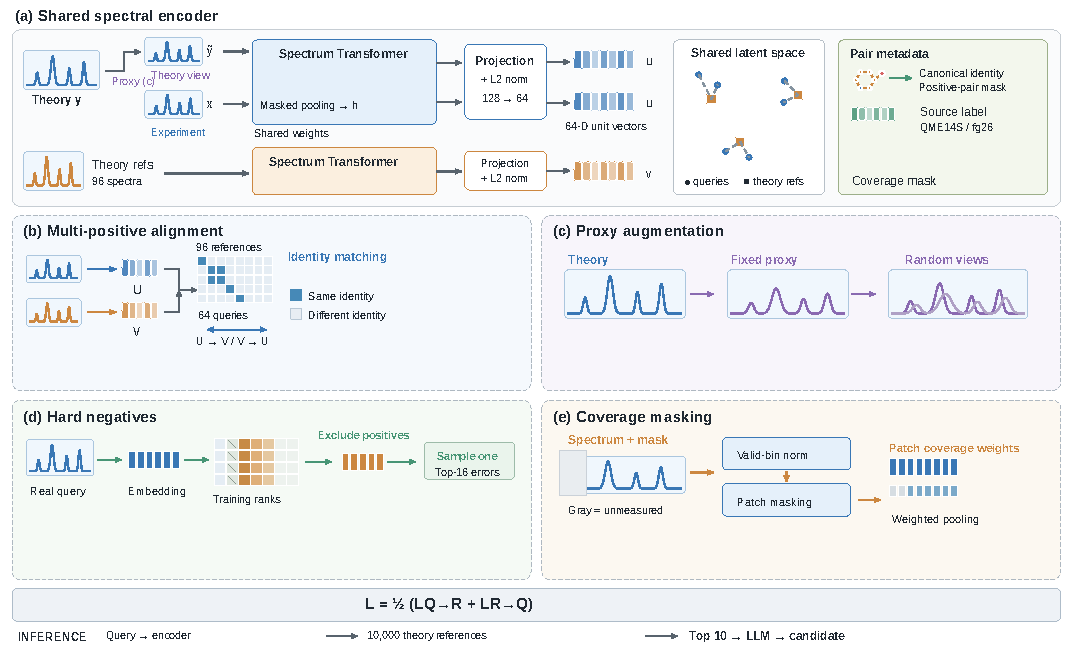
\includegraphics[width=\textwidth]{figures/raman_training_author_final.pdf}
\else
  \fbox{\begin{minipage}[c][0.50\textwidth][c]{0.96\textwidth}
    \centering\sffamily\color{gray}
    Training-method figure reserved\\[6pt]
    To be inserted after author finalization
  \end{minipage}}
\fi
\caption{Domain-adapted retrieval training. (a) A shared encoder embeds experimental queries, augmented theoretical queries and theoretical references. Blue circles and orange squares denote query and reference embeddings, respectively. (b) Contrastive learning aggregates probability over all same-identity positives. (c) Source-dependent proxies perturb frequency scale, shift and broadening. (d) Hard negatives are sampled from the top 16 incorrect training matches. (e) Coverage masks distinguish unmeasured regions from observed zeros and control normalization, attention and pooling. Proxy fitting, mining and encoder updates use training data only. All graphical examples are schematic.}
\label{fig:domain_training}
\end{figure*}

\subsection{What Is Adapted Across Domains?}\label{sec:proxy}
The transformation from a theoretical curve to a measurement can include a systematic shift in peak positions, different broadening, relative-intensity changes, baseline variation and incomplete instrument coverage. A global transformation cannot explain every molecule-specific change, but it gives an interpretable starting point for augmentation. We fit a source-dependent effective curve proxy and combine it with real spectral pairs, rather than requiring the proxy to reproduce the entire measurement process.

For source $s$, the three fitted parameters are scale $a_s$, translation $b_s$ and Gaussian width $\sigma_s$. The implementation smooths in the theoretical coordinate and then interpolates:
\begin{equation}\label{eq:proxy}
(T_{\phi_s}y)(\nu)=\frac{1}{a_s}
 (G_{\sigma_s}*y)\!\left(\frac{\nu-b_s}{a_s}\right),
\quad \phi_s=(a_s,b_s,\sigma_s).
\end{equation}
The $1/a_s$ factor preserves integrated intensity under the affine coordinate change. A Gaussian is truncated at four standard deviations; output locations are valid only when the corresponding kernel support lies within known theoretical coverage. This prevents artificial boundary values from becoming spectral evidence.

Parameters are estimated only from training pairs of the same molecular identity. For a source-specific set $\mathcal{P}_s$, let $\omega_i$ give equal total weight to each molecular group. We minimize
\begin{equation}\label{eq:proxyfit}
\phi_s^\star=\arg\min_{\phi\in\Phi}
\sum_{i\in\mathcal{P}_s}\omega_i
\bigl[1-\operatorname{cos}_{\Omega_i}(T_\phi y_i,x_i)\bigr],
\end{equation}
where $\Omega_i$ is a fixed, conservative common support valid under every bounded transformation. The fit cannot improve its score merely by moving difficult regions outside the mask. We use $a\in[0.94,1.06]$, $b\in[-40,40]$\,cm$^{-1}$ and $\sigma\in[0,12]$\,cm$^{-1}$. A coarse affine search initializes bounded derivative-free optimization. The frozen proxy used for encoder training exhausted its fitting budget and reached the broadening upper bound; these parameters are therefore an effective augmentation hypothesis, not converged estimates of instrument physics.

A single source mean underrepresents experimental variability. For each reliable training-pair affine fit, we store its joint scale/translation deviation from the source-specific median of reliable affine fits. Randomized views use no additional proxy transformation with probability 0.2, the fixed proxy with probability 0.2, and a perturbed proxy with probability 0.6. In the last case, half a sampled joint deviation is added to the source parameters and clipped to $\Phi$; the additional width is drawn uniformly between zero and the fixed width. Sampling a joint residual preserves observed scale/shift dependence without transplanting a different molecule's full residual spectrum. Reliability requires aligned correlation at least 0.25 and a correlation improvement of at least 0.05; sources with fewer than ten reliable fits use zero affine residuals.

All arms retain the same base positive-view augmentation, including small noise and contaminant peaks. Thus ``no additional proxy'' does not mean an unaugmented spectrum, and the fixed arm is not a pure physical simulator. A training experimental mask is sampled and intersected with transformed theoretical coverage. If fewer than 100 bins remain, the view falls back to its base augmentation and original coverage. No validation or test curve determines these transformations. Real experimental queries are also included directly in the loss, so deviations beyond the proxy family can affect the learned representation.

\subsection{Coverage-Aware Spectral Encoder}\label{sec:encoder}
All curves are interpolated by their physical coordinates onto 3,501 bins spanning 500--4000\,cm$^{-1}$. The associated Boolean mask distinguishes unavailable regions from measured zero intensity. For a valid-bin count $n_m=\sum_t m_t$, normalization uses only observed values:
\begin{align}
\mu_m&=n_m^{-1}\sum_t m_tx_t,\qquad
v_m=n_m^{-1}\sum_t m_t(x_t-\mu_m)^2,\\
\widetilde{x}_t&=m_t\frac{x_t-\mu_m}{\max(\sqrt{v_m},10^{-6})}.
\end{align}
Empty coverage is rejected. Without this distinction, zero padding changes the mean and variance according to measurement range, introducing a shortcut unrelated to molecular identity.

Overlapping 16-bin patches with stride 8 produce 436 tokens. A linear projection maps each patch to width 128; learned positional embeddings retain wavenumber location. Three pre-normalized Transformer layers use four attention heads, a fourfold feed-forward expansion, GELU and dropout 0.1. Entirely missing patches are excluded as attention keys and values. Let $w_p$ be the valid-bin fraction in patch $p$, and let $h_p$ be its final layer-normalized representation. We use coverage-weighted pooling and a two-layer projection:
\begin{equation}\label{eq:embedding}
\bar h=\frac{\sum_p w_ph_p}{\sum_p w_p},\qquad
z=\frac{W_2\operatorname{ReLU}(W_1\bar h)}
 {\|W_2\operatorname{ReLU}(W_1\bar h)\|_2}.
\end{equation}
Here $W_1$ maps 128 to 128 dimensions and $W_2$ maps 128 to 64; both are bias-free. Partially covered patches remain usable but contribute less to pooling. The same encoder processes experimental and theoretical spectra. Source labels determine training-view construction and sampling, but are not required as query-side encoder inputs at inference.

\subsection{Real Pairs, Multiple Positives and Hard Negatives}\label{sec:loss}
Each training step contains 32 augmented theoretical queries and 32 real experimental queries. Real pairs are sampled hierarchically by source, molecular identity and measurement, then matched to a same-identity reference from that source. This reduces domination by repeated measurements or the more common theoretical source. The reference batch contains 64 corresponding records plus 32 additional records; it is rectangular relative to the query batch.

Let $u_i$ and $v_j$ be query and reference embeddings, with identity labels $c_i$ and $d_j$. Define $P_i=\{j:c_i=d_j\}$ and $\ell_{ij}=u_i^\top v_j/\tau$, with $\tau=0.1$. The forward loss is
\begin{equation}\label{eq:contrastive}
\mathcal{L}_{Q\to R}=-\frac{1}{B_Q}\sum_i
\log\frac{\sum_{j\in P_i}\exp(\ell_{ij})}
 {\sum_{j=1}^{B_R}\exp(\ell_{ij})}.
\end{equation}
The reverse loss has the same form over references with at least one same-identity query; unsupported extra references are excluded from that reverse average. We optimize $\mathcal{L}=\tfrac12(\mathcal{L}_{Q\to R}+\mathcal{L}_{R\to Q})$. Summing the positive probability mass, rather than choosing only a diagonal match, avoids contradictory negative labels when a molecule has several theoretical records or appears repeatedly within a batch.

For the hard-negative arm, the encoder ranks training references for each training experimental query after every epoch. All references with the correct full identity are removed, and one additional reference is sampled from the 16 highest-ranked incorrect records for each of the 32 real queries. The first epoch uses random extras. Control arms also use 32 extra references, sampled randomly, so hard mining does not increase the per-step reference budget. These are model-confusable alternatives, not chemically certified negative peak assignments; the loss still determines positive membership globally by identity.

We use AdamW with learning rate $3\times10^{-4}$, weight decay $10^{-4}$ and gradient norm clipping at 1. Training runs for at most 40 epochs of 160 steps, with patience 8. Checkpoints are chosen by development group-weighted Exact@10, then Exact@1 and lower training loss. The four arms share initialization, real pairs, architecture, optimizer and reference budget. They differ in the theoretical domain view (empirical baseline, fixed proxy or random proxy) and extra-reference selection. Five-seed replication compares the empirical baseline with random proxy plus hard negatives using paired seeds 0--4.

\subsection{Spectral Evidence and a Constrained Final Decision}\label{sec:selection}
At inference, the learned similarity retrieves ten structures from the fixed theoretical index. The LLM receives an experimental peak table and candidate SMILES in retrieval order. It does not receive a target formula, target mass, true identity, candidate spectrum or similarity score. A prompt explicitly treats retrieval order as a useful prior while permitting a different choice based on peak evidence.

The optional knowledge stage matches detected peaks to frequency intervals and supplies textual vibrational assignments. The legacy knowledge base (KB) contains 181 rules and provides the matched evidence evaluated on Test-200. A separate 15-mode Raman library supports controlled development experiments. It combines source-backed frequency ranges with conservative project-defined SMARTS mappings for structural compatibility. These mappings are operational tests rather than independently validated assignments of every mode. Peaks within a 20\,cm$^{-1}$ tolerance can support a rule, but an undetected peak does not conclusively exclude a structure.

For a non-LLM control, a candidate's coverage score is the fraction of matched modes whose SMARTS are compatible with that structure. Ties retain retrieval order. A learned linear control combines inverse rank, 15 mode-compatibility indicators and coverage; it fits training-group pairwise Tanimoto differences with squared loss and $L_2$ regularization, selected on development data. Rank-only and rules-only variants isolate these feature families. These controls ask whether deterministic or fitted evidence integration explains any apparent LLM advantage.

The LLM is asked to output an index from 1 to 10, confidence and a brief explanation. Only the selected index determines the prediction. Deterministic normalization accepts an unambiguous final index or a uniquely matching candidate SMILES; conflicting or out-of-range choices remain invalid. There is no top-1 fallback, and normalization never accesses the target identity. Confidence is logged when present and does not trigger edits. The deployed policy never invents or modifies a candidate; output recovery is detailed in Section~\ref{sec:repro}.

% 功能概述：只保留支撑域适配、检索与候选判别主旨的最新完成结果。
% 主要职责：统一 Test-200、五种子、机制检查和规则对照；报告缺失样本与统计不确定性。
% 代码库关系：由 main.tex 引入；数值依据 results/jj-20260909 冻结快照，审稿逐项核对见 REVIEW_RESPONSE_AUDIT.md。
\section{Experiments}\label{sec:latest_experiments}
\subsection{Data, Identity Control and Evaluation Scope}\label{sec:protocol}
The main benchmark contains 200 experimental Raman queries from SDBS~\cite{sdbsAIST} and 10,000 unique theoretical reference structures. The theoretical records come from the QME14S and fg26 sources in the cached processed SpecGPT collection; they are not all QM9S records. The corrected protocol, ensures that every test target is present under full canonical/isomeric identity. An earlier version had 21 incomplete identity matches: 13 references were repaired and eight query/reference slots were replaced deterministically without retrieval-score selection. Direct-LLM outputs were refreshed for those eight queries; the other 192 were reused after input and request equality checks.

The current adaptation split has 601 experimental training spectra from 565 molecular groups and 149 development spectra from 142 groups. All 200 test groups are excluded from experimental training, proxy fitting and checkpoint selection. The original 9,500/500 theoretical partition is retained; nonprotected supplemental theoretical records extend the reference pool to 10,967 records for 10,704 identities. Development retrieval uses these 10,704 identities, each with one fixed indexed reference. Final test retrieval uses the original 10,000 identities. Theoretical records of development and test identities may be available during training: the protected item is the experimental observation, not every representation of its molecule.

This is therefore closed-library transfer to unseen experimental spectra of known identities. It does not measure unseen-molecule generalization. Test-200 has been inspected in successive experiments, despite being excluded from gradient updates and checkpoint selection; it is a fixed benchmark, not a newly blinded test. The earlier QM9S--ChEMBL study used different chemical support and unmatched 211/50/20-query batches. Its historical scores are excluded from the current main comparison rather than pooled with the corrected experiment.

\subsection{Metrics and Statistical Units}\label{sec:metrics}
Exact@$K$ tests full-structure equality with any of the first $K$ predictions; the Test-200 denominator is always 200. Development selection averages repeated spectra within each molecular group before averaging groups. Molecular parsing and fingerprint calculations use RDKit~\cite{landrum2013rdkit}. Tanimoto similarity uses radius-2, 2,048-bit Morgan fingerprints with bond types and without chirality. Consequently, a high Tanimoto score need not imply stereochemically exact identity.

Chemical graph edit distance (GED v2) uses atomic-number node labels and discrete bond-type edge labels. A bounded search applies a 10-second limit to each pair. Invalid or timed-out values remain missing; structural means report computable counts, and paired comparisons use common computable queries. Historical first-return GED upper bounds are excluded from the current comparison. Candidate-selection validity requires a unique legal index, whereas direct-generation validity requires a parseable SMILES. These rates therefore measure different output obligations rather than equivalent chemical-generation capabilities.

Five-seed summaries report sample standard deviations. A Student-$t$ interval on paired seed differences quantifies training randomness, with the seed as the independent repetition. Query-level or molecular-group bootstrap intervals assess paired prediction differences on a fixed checkpoint; they do not replace retraining. Development ablations are exploratory because their checkpoints and settings were selected on that data. All results below are the latest completed compatible artifacts collected on 9 September 2026; newer training checkpoints are not substituted into older frozen LLM candidate lists.

\subsection{Does Domain Adaptation Improve Retrieval?}\label{sec:retrieval_results}
\begin{table}[t]
\centering
\PaperTableSetup{\footnotesize}
\caption{Mechanism checks on the same development spectra}
\label{tab:mechanism}
\begin{tabularx}{\linewidth}{>{\raggedright\arraybackslash}Xrr}
\toprule
\rowcolor{HdrBg}
\multicolumn{1}{l}{\PaperHead{Configuration}} & \PaperHead{Hits@10} & \PaperHead{Group @10}\\[1pt]
\midrule
\PaperGroup{3}{RetBg}{Direct cosine: common support, no encoder}
\rowcolor{RetBg!55}Original theoretical curves & 8/149 & ---\\
\rowcolor{RetBg!28}Fixed proxy curves & 39/149 & ---\\
\PaperGroup{3}{AgtBg}{Paired encoder: controlled seed-0 training}
\rowcolor{AgtBg!55}Empirical domain augmentation & 73/149 & 51.06\\
\rowcolor{AgtBg!28}Fixed proxy + random extras & 77/149 & 52.82\\
\rowcolor{AgtBg!55}Random proxy + random extras & 77/149 & 52.82\\
\rowcolor{AgtBg!28}Random proxy + hard negatives & 80/149 & 54.58\\
\bottomrule
\end{tabularx}\arrayrulecolor{black}
\PaperNote{149 spectra, 142 groups; Group @10 is a percentage. The direct-curve control isolates proxy correction; encoder rows share real pairs, architecture, initialization and training budget.}
\end{table}

\paragraph{Curve correction before representation learning.}
Table~\ref{tab:mechanism} first compares direct cosine retrieval using original and fixed-proxy theoretical curves. Both scores use the same common support for each query--candidate pair. No development curve is fitted individually. Exact@10 rises from 8/149 to 39/149: 33 targets enter the top ten and two leave. The molecular-group-weighted gain is 21.13 percentage points (pp), with a paired bootstrap 95\% interval of $[14.08,28.87]$ pp. This is evidence that correcting the curve distribution can help identity retrieval even without a learned encoder. Its mask convention differs from the historical zero-filled cosine baseline, so those rates should not be directly subtracted.

\paragraph{Controlled encoder mechanisms.}
The four encoder arms in Table~\ref{tab:mechanism} keep the real-pair and multiple-reference protocol fixed. Fixed and random proxies each give 77/149 top-ten hits, while adding hard negatives gives 80/149. Group-weighted differences are small in this single seed: hard minus baseline is 3.52 pp with an exploratory group-bootstrap interval of $[-5.28,12.32]$ pp. Thus the table documents the effect sizes without establishing that each added mechanism independently improves generalization. The direct-curve control and encoder controls answer different questions; neither is a same-data contrastive-versus-noncontrastive loss ablation.

\begin{table}[t]
\centering
\PaperTableSetup{\footnotesize}
\caption{Test retrieval over five paired training seeds}
\label{tab:multiseed}
\begin{tabularx}{\linewidth}{>{\raggedright\arraybackslash}Xrrr}
\toprule
\rowcolor{HdrBg}
\multicolumn{1}{l}{\PaperHead{Training}} & \PaperHead{Exact@1} & \PaperHead{Exact@5} & \PaperHead{Exact@10}\\[1pt]
\midrule
\rowcolor{RetBg!55}Paired baseline & 15.50 $\pm$ 4.18 & 35.60 $\pm$ 4.13 & 46.30 $\pm$ 5.22\\
\rowcolor{AgtBg!55}Proxy + hard negatives & 19.50 $\pm$ 1.70 & 43.90 $\pm$ 1.98 & 53.60 $\pm$ 2.36\\
\bottomrule
\end{tabularx}\arrayrulecolor{black}
\PaperNote{Test-200, percentages; mean $\pm$ sample SD for seeds 0--4. The paired test @10 gain is 7.30 pp, 95\% $t$ interval $[-0.58,15.18]$ pp.}
\end{table}

\paragraph{Training randomness and source heterogeneity.}
The latest five-seed comparison is in Table~\ref{tab:multiseed}. Proxy plus hard negatives reaches 53.60\% mean Test-200 Exact@10, versus 46.30\% for the paired baseline, winning in four of five seeds. The paired mean-gain interval includes zero. Development group Exact@10 improves in all five seeds: 54.86\% $\pm$ 2.26\% versus 43.87\% $\pm$ 4.30\%, with a paired gain interval $[4.35,17.63]$ pp. These observations support a development-level effect and a higher test mean, not a statistically established test gain across training seeds. Seed 0 illustrates the uncertainty: baseline test @10 is 52.5\% and hard is 51.5\%.

Transfer also varies by theoretical source. Hard achieves 59.86\% $\pm$ 1.67\% @10 on 138 QME14S queries and 39.68\% $\pm$ 6.71\% on 62 fg26 queries. Relative to the paired baseline, the source-specific gain intervals are $[0.80,15.14]$ and $[-7.14,18.75]$ pp. The remaining gap is not explained by a single global frequency correction. Source, molecular composition and phase may be confounded, so these strata do not identify a causal physical mechanism.

The frozen single-seed hard encoder used for all downstream LLM tests retrieves 41/200, 87/200 and 103/200 targets at ranks 1, 5 and 10; zero-filled raw cosine kNN retrieves 1/200, 11/200 and 22/200. The five-seed checkpoints have not been evaluated with the LLM selector. A later proxy fit improves group-weighted validation cosine from 0.5036 to 0.7665 on 207 pairs, but the encoders used the earlier frozen fit. Improved later curve fit cannot be credited to their measured retrieval performance.

\subsection{Final Identification and the Remaining Selection Gap}\label{sec:selection_results}
\begin{table*}[t]
\centering
\PaperTableSetup{\small}
\caption{Overall molecular identification on corrected Test-200}
\label{tab:latest_main}
\begin{tabularx}{\linewidth}{>{\raggedright\arraybackslash}Xrrrr}
\toprule
\rowcolor{HdrBg}
\multicolumn{1}{l}{\PaperHead{Method}} & \PaperHead{Valid $\uparrow$} & \PaperHead{Exact $\uparrow$} & \PaperHead{Tanimoto $\uparrow$} & \PaperHead{Chemical GED $\downarrow$}\\[1pt]
\midrule
\PaperGroup{5}{RetBg}{Pretrained competing methods}
\rowcolor{RetBg!55}Vib2Mol retrieval + Raman reranking & 100.0 & 0.0 & 0.0644 (200) & 12.5667 (150)\\
\rowcolor{RetBg!28}VibraCLIP, no mass & 100.0 & 0.0 & 0.0490 (200) & 9.9457 (184)\\
\rowcolor{RetBg!55}Vib2Mol generation + Raman reranking & 81.0 & 0.0 & 0.0582 (162) & 9.1698 (159)\\
\rowcolor{RetBg!28}MolSpectLLM (Raman unavailable) & N/A & N/A & N/A & N/A\\
\PaperGroup{5}{RetBg}{Retrieval}
\rowcolor{RetBg!55}Raw cosine kNN & 100.0 & 0.5 & 0.1132 (200) & 8.1778 (180)\\
\rowcolor{RetBg!28}Frozen hard encoder top-1 & 100.0 & 20.5 & 0.3205 (200) & 5.3057 (193)\\
\PaperGroup{5}{DirBg}{Direct generation}
\rowcolor{DirBg!55}Direct DeepSeek & 99.0 & 2.5 & 0.1946 (198) & 6.3011 (186)\\
\PaperGroup{5}{AgtBg}{Candidate selection}
\rowcolor{AgtBg!55}kNN + DeepSeek & 100.0 & 4.0 & 0.1598 (200) & 7.4213 (178)\\
\rowcolor{AgtBg!28}Frozen hard encoder + DeepSeek & 100.0 & 22.0 & 0.3515 (200) & 5.0258 (194)\\
\PaperGroup{5}{KnwBg}{Full Agent: frozen hard encoder + legacy KB + model}
\rowcolor{KnwBg!55}GPT-5~\cite{gpt-5} & 100.0 & 18.5 & 0.3082 (200) & 5.4603 (189)\\
\rowcolor{KnwBg!28}o3~\cite{o3_and_o4-mini} & 100.0 & 20.5 & 0.3352 (200) & 5.0890 (191)\\
\rowcolor{KnwBg!55}Claude Sonnet 4.6~\cite{claude-sonnet-4-6} & 99.5 & 29.0 & 0.4207 (199) & 4.4404 (193)\\
\rowcolor{KnwBg!28}Gemini 2.5 Flash~\cite{gemini2-5} & 100.0 & 16.5 & 0.2985 (200) & 5.4688 (192)\\
\rowcolor{KnwBg!55}DeepSeek v4 Flash-Ascend~\cite{deepseek2026deepseek} & 100.0 & 22.0 & 0.3575 (200) & 5.0785 (191)\\
\bottomrule
\end{tabularx}\arrayrulecolor{black}
\PaperNote{Valid and top-1 Exact are percentages; parentheses give computable counts. GED means use different subsets. All encoder-selection rows use the frozen seed-0 model. Full-Agent validity is measured after output recovery (Section~\ref{sec:repro}), not initial format compliance; token budgets differ across attempts. Competing checkpoints do not receive SpectraExpert's experimental adaptation pairs; VibraCLIP omits 85 failed conformers, none a query target. N/A denotes unavailable Raman predictions, not zero accuracy.}
\end{table*}

Table~\ref{tab:latest_main} compares final identification on the same 200 experimental queries. Candidate-only DeepSeek achieves 44 exact matches, a net gain of three over retrieval top-1. It corrects 15 predictions but loses 12 previously correct predictions; 29 remain correct and 144 remain incorrect. Table~\ref{tab:selection_gap} separates failures caused by missing candidates from failures after successful retrieval, following Eq.~\eqref{eq:ceiling}.

\begin{table}[t]
\centering
\PaperTableSetup{\footnotesize}
\caption{Selection outcomes within the frozen top ten}
\label{tab:selection_gap}
\begin{tabularx}{\linewidth}{>{\raggedright\arraybackslash}Xrrr}
\toprule
\rowcolor{HdrBg}
\PaperHead{Decision rule} & \PaperHead{Correct} & \PaperHead{Missed} & \PaperHead{Success \%}\\[1pt]
\midrule
\rowcolor{RetBg!55}Retrieval top-1 & 41 & 62 & 39.81\\
\rowcolor{AgtBg!55}DeepSeek, no KB & 44 & 59 & 42.72\\
\PaperGroup{4}{KnwBg}{Full Agent with legacy KB}
\rowcolor{KnwBg!55}GPT-5 & 37 & 66 & 35.92\\
\rowcolor{KnwBg!28}o3 & 41 & 62 & 39.81\\
\rowcolor{KnwBg!55}Claude Sonnet 4.6 & 58 & 45 & 56.31\\
\rowcolor{KnwBg!28}Gemini 2.5 Flash & 33 & 70 & 32.04\\
\rowcolor{KnwBg!55}DeepSeek v4 Flash-Ascend & 44 & 59 & 42.72\\
\bottomrule
\end{tabularx}\arrayrulecolor{black}
\PaperNote{The target is present for 103/200 queries and absent for 97/200 in every row. Correct + Missed = 103; Success = Correct/103. Missed includes any invalid choice on a retrievable query. Full-Agent results follow the output-recovery policies in Section~\ref{sec:repro}; this is a decomposition of existing predictions, not a new experiment.}
\end{table}

Against direct LLM generation, encoder plus LLM improves exact accuracy by 19.5 pp, with a paired query-bootstrap interval $[14.0,25.5]$ pp. Chemical GED improves by 1.221 on 181 common computable queries, interval $[0.547,1.901]$. This comparison establishes a benefit for the full retrieval-assisted pipeline under its available supervision. It does not isolate the reasoning module, since the pipeline supplies known candidate structures and an experimentally adapted retriever.

For DeepSeek, adding matched legacy knowledge preserves 44/200 exact matches, with 13 gains and 13 losses relative to candidate-only selection. Its Tanimoto mean rises slightly while its GED means do not improve; the differing computable subsets also limit direct interpretation of these means. Thus there is no net exact-match gain from this knowledge intervention. Choosing the minimum-GED or maximum-Tanimoto candidate among all ten has not been comprehensively audited.

\paragraph{Model substitution with frozen evidence.}\label{sec:agent_models}
The five full-Agent conditions share the same queries, candidate order and matched legacy KB. After output recovery, exact accuracy ranges from 16.5\% for Gemini to 29.0\% for Claude. Claude gains 23 exact predictions and loses six relative to retrieval top-1. Its paired advantage over DeepSeek is 7.0 pp, with an exploratory query-bootstrap 95\% interval of $[2.5,12.0]$ pp. Nevertheless, Claude misses 45 retrievable targets, alongside 97 targets absent from the shortlist. The comparison measures model substitution under recorded recovery policies; it does not isolate knowledge effects or equalize inference budgets. The four replacement models lack matched direct-generation and no-knowledge controls.

\subsection{Knowledge and Non-LLM Ablations}\label{sec:ablations}
\begin{table}[t]
\centering
\PaperTableSetup{\footnotesize}
\caption{Same-query development ablations}
\label{tab:kb}
\begin{tabularx}{\linewidth}{>{\raggedright\arraybackslash}Xrrr}
\toprule
\rowcolor{HdrBg}
\multicolumn{1}{l}{\PaperHead{Configuration}} & \PaperHead{Exact} & \PaperHead{Group \%} & \PaperHead{Tanimoto}\\[1pt]
\midrule
\PaperGroup{4}{RetBg}{Shared 15-mode controls}
\rowcolor{RetBg!55}Retrieval top-1 & 16/149 & 10.56 & 0.3282\\
\rowcolor{RetBg!28}Retrieval + rule coverage & 10/149 & 7.04 & 0.2585\\
\rowcolor{AgtBg!55}Retrieval + LLM & 19/149 & 13.38 & 0.3446\\
\rowcolor{AgtBg!28}Retrieval + modes + LLM & 21/149 & 14.08 & 0.3355\\
\PaperGroup{4}{KnwBg}{Knowledge representation controls}
\rowcolor{KnwBg!55}LLM, matched legacy KB & 22/149 & 14.44 & 0.3703\\
\rowcolor{KnwBg!28}LLM, static full legacy KB & 22/149 & 14.79 & 0.3558\\
\rowcolor{KnwBg!55}LLM, short mode evidence & 19/149 & 13.03 & 0.3382\\
\rowcolor{KnwBg!28}LLM, filtered full modes & 17/149 & 11.62 & 0.3019\\
\rowcolor{KnwBg!55}LLM, filtered short modes & 18/149 & 11.62 & 0.3062\\
\bottomrule
\end{tabularx}\arrayrulecolor{black}
\PaperNote{Identical 149 spectra, 142 groups, frozen candidates and peak extraction; all LLM arms use DeepSeek. All choices are valid. Group percentages and spectrum-weighted Tanimoto use different averaging units.}
\end{table}

The first four rows of Table~\ref{tab:kb} form the requested retrieval/rules/LLM/combined comparison on common development data. Full mode evidence adds only 0.70 pp group-weighted exact accuracy to the no-KB LLM, with interval $[-5.63,6.69]$ pp. Its group-weighted Tanimoto difference is $-0.01051$, interval $[-0.06368,0.04316]$. On 138 queries with computable chemical GED in all four arms, means are 4.5725, 5.3043, 4.5362 and 4.2971, respectively. A separate paired comparison of the two LLM arms over their 140 common queries gives a group-weighted GED improvement of 0.2657 with interval $[-0.3659,0.9273]$. These intervals do not establish a stable knowledge benefit.

Matched legacy and static full knowledge both obtain 22/149 exact matches. The static condition appends the full legacy Markdown without query matching or candidate filtering; it was run later using the earlier no-KB responses as a control. The short mode condition changes both wording and the number of evidence records, while candidate filtering also introduces compatibility mappings. These are joint prompt interventions, not pure prompt-length or single-factor causal experiments. Filtering decreases exact hits to 17 or 18 and therefore cannot be assumed beneficial.

\begin{table}[t]
\centering
\PaperTableSetup{\footnotesize}
\caption{Frozen non-LLM controls on Test-200}
\label{tab:nonllm}
\begin{tabularx}{\linewidth}{>{\raggedright\arraybackslash}Xrrr}
\toprule
\rowcolor{HdrBg}
\multicolumn{1}{l}{\PaperHead{Method}} & \PaperHead{Exact} & \PaperHead{Tanimoto} & \PaperHead{GED ($n$)}\\[1pt]
\midrule
\rowcolor{RetBg!55}Retrieval top-1 & 41/200 & 0.3205 & 5.3057 (193)\\
\rowcolor{RetBg!28}Rule coverage & 22/200 & 0.2347 & 6.6684 (187)\\
\rowcolor{KnwBg!55}Linear rank only & 41/200 & 0.3205 & 5.3057 (193)\\
\rowcolor{KnwBg!28}Linear rules only & 23/200 & 0.2709 & 5.8639 (191)\\
\rowcolor{KnwBg!55}Linear rank + rules & 41/200 & 0.3205 & 5.3057 (193)\\
\bottomrule
\end{tabularx}\arrayrulecolor{black}
\PaperNote{All methods choose from the same frozen top ten. GED is chemical GED v2; Tanimoto uses all 200 predictions. Linear rank and rank + rules preserve every top-1 prediction.}
\end{table}

The trained non-LLM controls in Table~\ref{tab:nonllm} use regularization selected from $\{0.01,0.1,1,10,100\}$. Rules alone degrade exact accuracy; combining them with rank leaves every retrieval top-1 decision unchanged on both development and test data. Coverage reranking changes 145 test decisions, with seven exact gains and 26 losses: a net $-9.5$ pp, interval $[-15.0,-4.0]$ pp. On the 179 queries jointly computable for retrieval, coverage, rules-only linear and rank-plus-rules linear, GED means are 5.4134, 6.8045, 5.8715 and 5.4134. These controls reject the assumption that coarse rule agreement automatically resolves the candidate set.

There are two limits to this ablation. First, training candidates are not out-of-fold, and their 94.84\% top-ten coverage is much higher than development or test coverage. Second, the complete same-rule four-arm design is available on development data only. Test-200 includes a legacy-KB LLM condition, whereas the non-LLM controls use the 15-mode library; these rows do not constitute a fully matched four-arm test experiment.

\subsection{Competing Methods Under the Same Query Protocol}\label{sec:competitors}


Vib2Mol and VibraCLIP use the same query identities, candidate semantics and final scorer in the overall comparison (Table~\ref{tab:latest_main}). Model-specific preprocessing is retained: Vib2Mol resamples to 1,024 points with clip/max normalization, and VibraCLIP to 1,750 points with min--max normalization. Neither receives the true target formula or molecular mass. Vib2Mol uses its Raman--Kekul\'e-SMILES checkpoints; generation has beam size ten and reranks the first five outputs. VibraCLIP's no-mass checkpoint indexes 9,915 structures after 85 conformer failures, none involving a test target.

All three competitor branches have zero top-1 exact matches. VibraCLIP retrieves one target at ten and two at 25, while Vib2Mol retrieval finds one at 25; generation has no exact match in its ten beams. Low transfer accuracy must be interpreted alongside successful native-protocol checks. Our collected reproductions obtain 97.17\% Raman top-1 for Vib2Mol retrieval without formula and with reranking, and 62.59\% native top-1 for the VibraCLIP all-pairs no-mass checkpoint. These native rates use different datasets and candidate pools and are sanity checks, not rows in the unified ranking. Removing Vib2Mol reranking or using a fixed mean-mass anchor with VibraCLIP does not improve test exact @10. The result identifies a difficult transfer setting for these available checkpoints; it does not establish that their methods cannot adapt successfully with matched training resources.

No compatible MolSpectLLM Raman run is present in the collected artifacts. Its public description covers NMR, IR and MS rather than a matching Raman inference protocol. Its row in Table~\ref{tab:latest_main} is therefore N/A; zero accuracy or an original-paper score would not represent this benchmark. A complete comparison still requires a compatible implementation and equalized experimental adaptation.

% 功能概述：集中回应审稿人提出的失败机制、输出可靠性、复现参数与运行成本。
% 主要职责：区分已完成证据、当前政策变更及尚未验证的假设；不补造实验结果。
% 代码库关系：由 main.tex 引入；耗时来自 results/jj-20260909/latency_audit.json 的只读日志聚合。
\section{Discussion and Practical Reproducibility}
The results identify two distinct constraints on closed-library Raman identification. Domain adaptation raises mean candidate recall, but successful retrieval still leaves substantial ambiguity for the selector. Even Claude, the strongest observed selector, resolves only 56.31\% of retrievable queries under the recorded recovery policy. Improving retrieval alone therefore cannot ensure reliable final identification, while selection cannot recover identities absent from the shortlist. This distinction connects the domain-adaptation experiments to the model and knowledge comparisons without attributing all pipeline gains to LLM reasoning.
\subsection{Why Rules and Structural Modification Can Fail}\label{sec:limits}
The rule-coverage control reveals an ambiguity mechanism: many distinct structures satisfy the same broad vibrational assignments. In Test-200, 134 queries have ties for maximum coverage, and the mean number of matched modes is 7.385. For query 3706, the correct top-ranked structure, \texttt{COC(C)(C)CC(C)=O}, has coverage 0.375, whereas the incorrect rank-six structure \texttt{CC=C1OC1CC} scores 0.5. Maximizing broad compatibility therefore discards an exact match. This is a concrete counterexample to coverage as a sufficient decision rule, not a causal explanation of every LLM mistake.

Coarse peak evidence can underdetermine a precise molecular edit, and self-reported confidence supplies no independently calibrated gate. The current experiment therefore evaluates candidate selection only, without the historical MODIFY branch.

The current mitigation disables MODIFY, requires a legal candidate index and validates the selected structure independently. It prevents free-form chemical-syntax failures but cannot guarantee identification: candidate-only DeepSeek loses 12 correct retrieval predictions, while full-Agent Claude loses six. A confidence-based preserve-or-edit policy and chemical verification loop would require separate calibration before any accuracy claim.

Current output failures separate two mechanisms: reasoning can exhaust the response budget, and a nonempty answer can violate the requested field syntax. Additional budget recovers empty GPT-5 and o3 answers; deterministic extraction recovers Gemini's final choices without changing their molecular selections. These repairs improve scoreability, not demonstrated reasoning accuracy, and do not explain historical unmatched direct-generation results.

\subsection{Inference Contract and Reproduction Details}\label{sec:repro}
The candidate-selector system prompt is fixed as follows; line breaks separate the requested output fields:
\begin{quote}\small\raggedright
You are an expert in Raman spectroscopy and molecular structure identification.
Select exactly ONE molecule from the provided candidate list using the experimental Raman peaks.
Candidates are ordered by decreasing retrieval similarity. This ordering is a useful prior, not a guarantee.
Use the peak evidence and structural compatibility; theoretical and experimental Raman spectra may differ.
Do not invent, modify, or combine candidates. Even when uncertain, choose the best available candidate.
End your response with these fields:\\
\texttt{SELECTED\_INDEX: <one integer from 1 to 10>}\\
\texttt{CONFIDENCE: <number from 0 to 1>}\\
\texttt{EXPLANATION: <brief justification referring to spectral evidence>}
\end{quote}
The user payload is ``Experimental Raman peaks (\{count\} peaks)'', followed by the formatted peak table; ``Ten candidate SMILES (retrieval order)'', followed by the numbered list; and ``Select exactly one candidate from this list.'' Knowledge conditions append their recorded evidence to this common input. The candidate-only condition omits it. Peak extraction uses the shared detector with relative height 0.05, relative prominence 0.02, distance 5, width 1 and z-score preprocessing. The final normalized index must be unique and lie in 1--10; no response is retried because its chemical prediction is wrong.

Direct generation uses \texttt{deepseek-v4-flash}. Candidate-only runs record Flash and Flash-Ascend routes: 93 successful earlier-route responses are reused and 307 later-route responses complete the two 200-query arms. Later knowledge runs use Flash-Ascend. The routes were treated as aliases operationally, but model equivalence has not been independently established. All these runs use temperature 0.2 and a 4,096-token output limit. No server-side generation seed is fixed, so training seeds 0--4 do not make API sampling reproducible. Each stored request preserves the requested route, and each response preserves the returned model identifier.

The four replacement-model Agent runs retain these frozen inputs and initially request the same temperature and output limit. Initial strict-field compliance is 50/200 for GPT-5, 122/200 for o3, 199/200 for Claude and 3/200 for Gemini. All 150 empty GPT-5 answers are retried with a 32,768-token limit. The 78 empty o3 answers are retried at 16,384 tokens, with one requiring a further 32,768-token attempt. Existing nonempty answers are retained. Gemini's 200 nonempty responses become scoreable through unambiguous final-answer extraction, without additional API calls. The same extraction rules preserve existing legal choices in the other models. Conflicts are rejected rather than resolved using ground truth. Effective validity therefore differs from initial compliance, and the repaired results do not represent independent, uniform-budget repeats.

The repository, \url{https://github.com/AndrewLuan/SpectraExpert}, preserves exact prompts, requests, decoding parameters, parsers, candidates, raw responses and source hashes. SHA-256 prefixes identify the corrected data manifest (\texttt{422e6729cad919b7}) and frozen encoder (\texttt{023da9724091f58a9}). The accompanying result audit records full hashes, run paths and the repaired-model summary. This separates replayable local retrieval from inference requiring continued access to proprietary services.

\subsection{Measured Resource Use and Remaining Scope}\label{sec:cost}
The four seed-0 encoder runs each complete in approximately 501--532 seconds on the recorded server execution. This measures training under that run's hardware and load, not a universal runtime. A 10,000-by-64 float32 reference index occupies 2.56 MB before metadata and requires 640,000 multiply--accumulate terms for one dense similarity query after encoding. These operation counts characterize the small final ranking stage; they do not measure peak extraction or encoder latency.

The two DeepSeek candidate-only arms report usage for all 400 received responses. Encoder and kNN candidate selection consume 1,094.19 and 1,093.26 total tokens per query, respectively. Their successful-attempt median latencies are 21.27 and 20.73 seconds, with 95th percentiles of 46.32 and 42.96 seconds. These service-call durations exclude queueing, failed attempts, retrieval and parsing; complete usage totals remain in the accompanying audit.

The logs also contain 187 earlier HTTP 403 attempts without reported usage, and interrupted requests without received responses have unknown usage. The replacement-model archive includes initial and repair attempts, token totals and successful-attempt latency summaries; the reused DeepSeek full-Agent usage is unavailable. Reported tokens are not guaranteed to equal billed consumption. Monetary costs and complete end-to-end latency have not been measured; no price is inferred. Retrieval top-1 avoids API calls and obtains 41/200 exact matches, compared with 33--58 across full-Agent models. Model-dependent gains and recovery overhead therefore matter for deployment, although these measurements do not determine an optimal operating policy.

All experimental observations originate from SDBS, so transfer across independent instruments or to unseen molecular identities remains untested. Five-seed test gains remain uncertain, API sampling is unreplicated, and the same-rule test ablation and matched competitor adaptation remain incomplete. A new experimental holdout would test whether retrieval gains survive further domain shifts. Repeated, equal-budget LLM runs with matched knowledge controls would distinguish reproducible selection gains from model, prompt and recovery-policy effects. The current evidence supports development retrieval gains and model-dependent identification within the fixed benchmark.


\section{Conclusion}
SpectraExpert separates theory--experiment retrieval from constrained molecular identification within a closed reference library. Paired adaptation with source-dependent proxies and identity-aware negatives improves development retrieval, while the five-seed test gain remains uncertain. Final identification depends on both candidate coverage and selector choice; even the best observed selector leaves many retrievable targets unresolved. Broad rule compatibility does not reliably resolve this ambiguity, and DeepSeek knowledge controls show no stable additional benefit. These findings support evaluating retrieval, selection and evidence integration separately when developing spectroscopy agents. Independent experimental data, matched competitor adaptation and repeated LLM evaluations are needed to establish transferability and reproducible end-to-end gains.

% 参考文献跨页时，仅在末页启动双栏平衡，避免前页纵向溢出。
\IEEEtriggeratref{23}
\IEEEtriggercmd{\balance}
\bibliographystyle{IEEEtran}
\bibliography{ref/ref}
\end{document}
